% Minimalistic template for a generic article, geared towards MDPI guidelines
% Use PDFLaTeX
\documentclass[a4paper,10pt]{article}
% Packages provided by the MDPI template already
\usepackage[T1]{fontenc}
\usepackage[utf8]{inputenc}
\usepackage{lineno}
\usepackage{microtype}
\usepackage{amsmath}
\usepackage{indentfirst}

% Custom packages
\usepackage[acronym,toc,shortcuts,nohypertypes=acronym]{glossaries}
\usepackage[colorlinks, allcolors=blue, unicode]{hyperref}
\usepackage{hyperxmp} % Import license metadata
\usepackage{titling} % Get the author for the metadata
\usepackage{textcomp} % \texttimes
\usepackage[pdf]{graphviz} % Importing dot files; can be replaced with generated PDFs
%\usepackage{dot2texi}

% Track changes package, remove when final; using a drop-in rather than the old version in TeX Live
% Usage: \added, \deleted, \replaced{new}{old}, \highlight, \comment
% All followed by an optional [id=<your id>, comment=<some comment>]
\usepackage[xcolor={usenames,dvipsnames}]{changes}
\definecolor{gem}{HTML}{003300}
\definechangesauthor[color=gem]{dm}
\definechangesauthor[color=NavyBlue]{jv}
\definechangesauthor[color=Purple]{nt}
\definechangesauthor[color=Mahogany]{mh}

% My own definition for the sections that start with a bold name but don't appear in TOC
\newcommand{\minisection}[1]{\medskip \textbf{#1:}}


% Metadata
\title{Fractional land cover classification method assessment using PROBA-V satellite data}
\author{Dainius Masiliūnas, Nandin-Erdene Tsendbazar, Martin Herold, \\ Myroslava Lesiv, Jan Verbesselt}
% * <Dainius Masiliūnas> 11:20:08 26 Mar 2019 UTC+0100:
% TODO: fix newline issue

\hypersetup{
    pdflicenseurl={http://creativecommons.org/licenses/by-sa/4.0/},
    pdfcopyright={This work is licensed under the Creative Commons Attribution-ShareAlike 4.0 International License.},
    pdfauthor={\theauthor}, % These are supposed to be the default but don't seem to be
    pdftitle={\thetitle},
    pdflang={en-GB}
}

% Acronyms - cite with \ac{}
\newacronym{GNSS}{GNSS}{Global Navigation Satellite System}
\makenoidxglossaries

% Use \begin{equation} for maths

\begin{document}

\maketitle

\linenumbers

\abstract{
The current common practice for producing global land cover maps is to represent land cover classes as discrete units, e.g. a pixel may be labelled as grassland, tree cover, or open water. However, in reality, the area covered by the pixel is hardly ever homogeneous, it may be e.g. trees surrounded by grass next to water. This mismatch between the reality and its representation in maps causes a loss in precision, as only the dominant land cover class can be represented in such ``hard'' classification maps. This problem is worse for coarse resolution land cover maps. A common workaround to this issue is to define mosaic classes, i.e. land cover classes that are combinations of other land cover classes, such as open forest (combination of grassland and tree cover). However, this approach leads to increasingly complex map legends and confusion about the definitions.

Our proposed solution to this issue is to employ fractional land cover mapping: for each pixel, define the proportion of the pixel that each considered land cover class occupies. This allows expressing an open forest as e.g. 40\% grassland, 60\% tree cover, and 0\% of the rest of the land cover classes. This ``fuzzy'' classification not only allows to more precisely express the land cover that exists in reality, but also gives users the flexibility to derive their own maps with a customised legend. For instance, if a user defines open forest as one that has less than 50\% tree cover and at least 30\% of grassland, they can generate a map with this definition from land cover fraction data, rather than relying on the definition that the mapmakers provide.
Exhaustive land cover fraction data is desired by a number of user communities, but to date there is no single global nor continental scale map that would provide fractions of each common land cover class.

In this paper, we tested the application of fractional land cover mapping over the continent of Africa. We compared the performance of four very different machine learning algorithms: random forest regression, multilayer perceptron neural networks, partial least squares regression, fuzzy nearest prototype classification and logistic regression. In order to allow the algorithms to make good predictions about land cover fractions, six types of covariates were used: spectral bands and vegetation indices derived from the Proba-V 100 m TOC reflectance data; temporal features derived from the full time series of said imagery; terrestrial features from a digital elevation model; soil properties and climate data from global models, and location. We compared the contribution of each of the covariate types to improving the accuracy of the model predictions.

One challenge when dealing with fractional data is the data imbalance: in most locations, only a single or a few classes dominate a pixel, with the rest taking up 0\% of the pixel. Values at the extremes (0\% and 100\%, i.e. pure pixels) are difficult for machine learning algorithms to estimate. We propose a new solution to this problem by combining three models: two classification models and one regression model. The first classification model determines whether a pixel is pure, and if so, it is processed using a classification model, otherwise it is processed with a regression model.

% Validation
% - 28k points
% - Independent training and validation sets

The models were trained on 26668 training points throughout Africa. The training points, collected as part of the Copernicus Global Land System: Dynamic Land Cover (CGLS-LC100) project, describe the fraction that each land cover class (bare soil, crops, grassland, shrubs, trees, urban/built-up, water and wetlands) occupies within a 100\texttimes100 m area, which is aligned to the grid used for Proba-V 100 m products. After the models were trained, their land cover class fraction predictions were compared with an independent validation set of 3617 points, which are likewise aligned to the Proba-V grid. Overall as well as per-class RMSE, MAE, and ME statistics were used to compare the models. In addition, the subpixel confusion-uncertainty matrix was used to analyse which classes were the most difficult to separate for each model, as well as to derive overall, users' and producers' accuracies and the kappa statistic. The models were compared with each other, as well as against a control intercept-only model.

Preliminary results show that the three-model approach increases the overall accuracy of the predictions by more accurately modelling the extreme values. From the machine learning models that were compared, random forest regression reaches the highest overall accuracy of 71\%. This is comparable to the reported accuracies of the current ``hard'' global land cover maps. Covariate importance analysis shows that spectral covariates are the most important for predicting land cover fractions, followed by the location, terrestrial and temporal covariates.

The application of the method on data gathered throughout Africa shows the applicability of the method to a variety of land cover conditions, ranging from highly heterogeneous agricultural landscapes to homogeneous bodies of water. Given enough reference data from other parts of the world and enough computational power, the method could be applied globally to upscale it to a global fractional land cover map. Such a map would cater to users with different fields of focus. Among other benefits, more precise estimation of land cover allows for 1) improved climate models to help reach Sustainable Development Goals (for which land cover is a key variable), 2) facilitate the making of models for vegetation and urban area dynamics, and 3) help governments and land owners keep better track of relevant land cover and its change. In addition, this work contributes to the operationalisation of the CGLS-LC100 project, which aims to produce exhaustive global land cover fractions as an operational product.

\minisection{Keywords} Fuzzy land cover classification, machine learning, random forest, gradient boosting, neural networks, fuzzy c-means, PROBA-V
}

\section{Introduction}

\begin{enumerate}
 \item Relevance of fractional LC mapping (link to user requirements and SDGs)
 \item Studies that have looked into fractional LC mapping so far
 \item Available fractional methods that were introduced in literature (wavelet transform etc.)
 \item Methods that are tested in this paper
\end{enumerate}

\added[id=dm]{
\textbf{Objectives}:
}

\begin{enumerate}
 \item Compare the performance of a variety of machine learning models for a continental-scale fractional land cover mapping task
 \item Compare the importance of covariates and covariate groups for the prediction of land cover fractions
 \item Investigate methods for reducing bias in the predictions with regards to zero inflation and predictions tending towards the mean
\end{enumerate}


\section{Materials and Methods}

\subsection{Reference data}

Description of the CGLOPS data, mentioning the balance and zero inflation problems, and the fact that the study area is Africa

\subsection{Covariates/Features}

\begin{enumerate}
 \item GLSDEM
 \item Proba-V time series
 \item SoilGrids and LandGIS
 \item WorldClim
\end{enumerate}

\subsection{Preprocessing}

\begin{enumerate}
 \item Temporal cloud filter for Proba-V
 \item Harmonic metrics extraction
 \item Terrain metrics calculation
 \item Additional climate parameter calculation
 \item Manual model feature selection
\end{enumerate}

\begin{figure}
 %\inputdigraph[width=\textwidth]{article-figures/algorithms}{dot}
 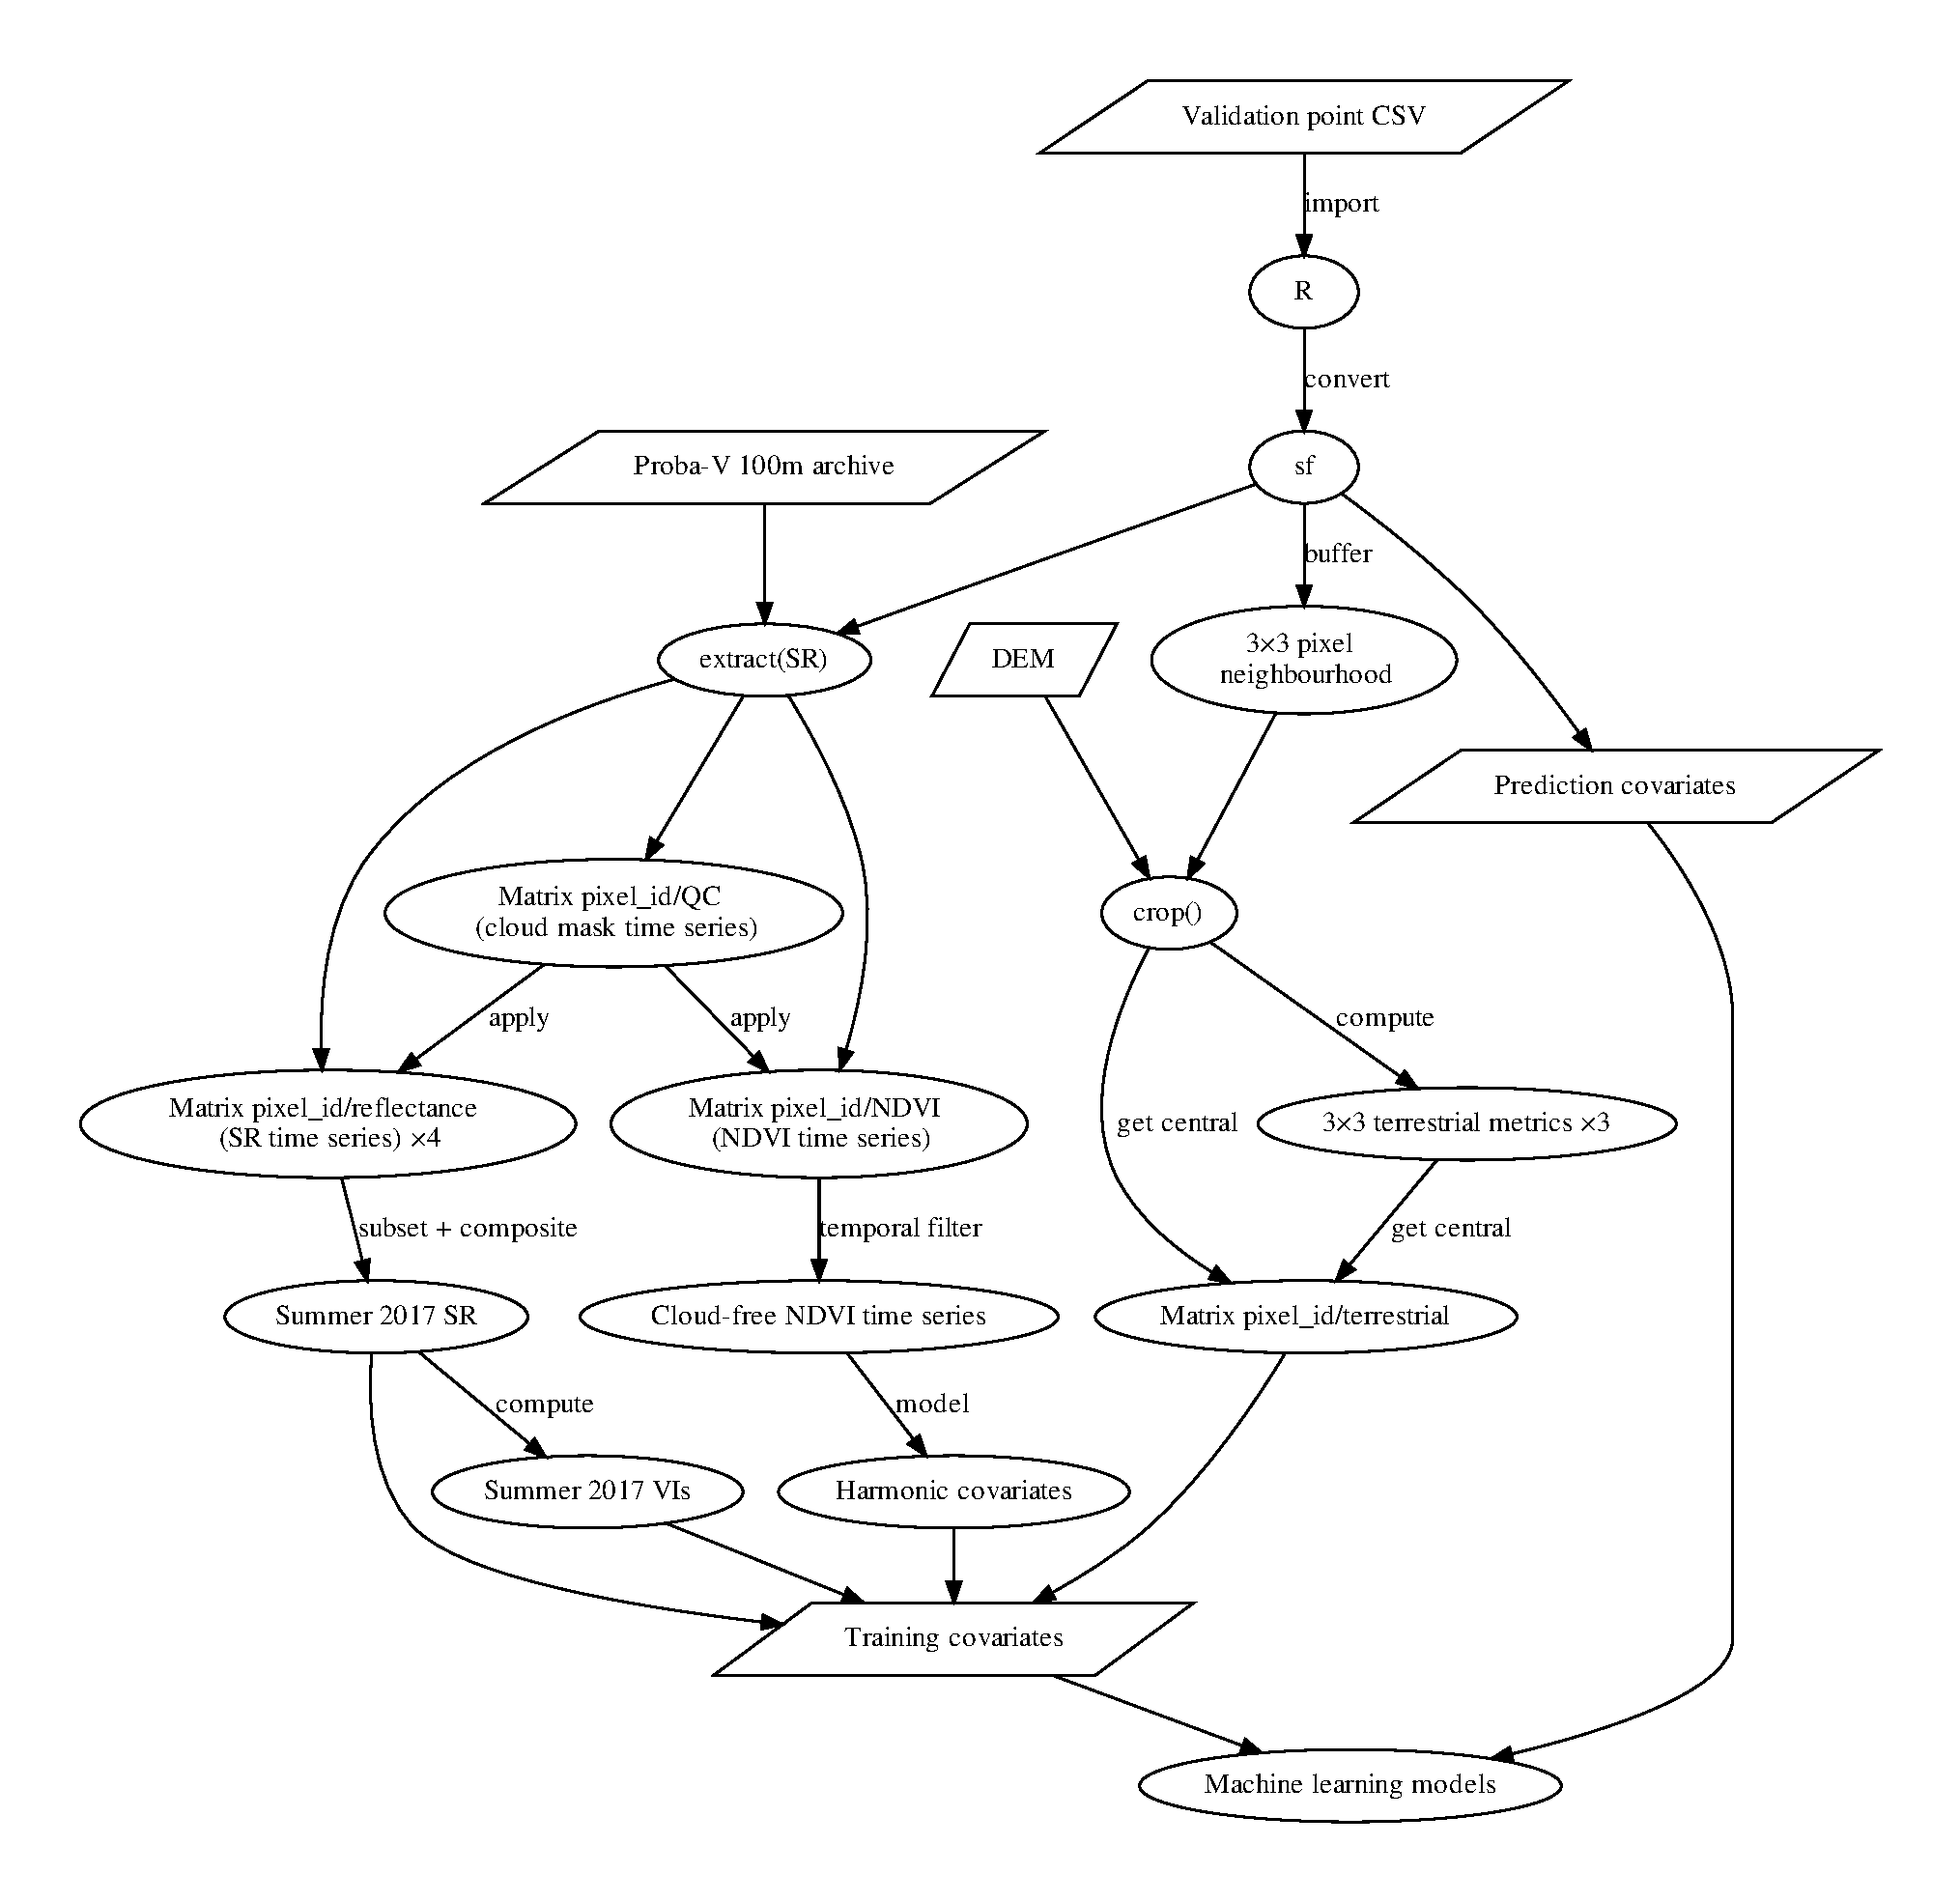
\includegraphics[width=\textwidth]{article-figures/algorithms}
 \caption{Preprocessing chain.}
\end{figure}


\subsection{Fractional land cover mapping methods}

\subsubsection{Logistic regression}

\subsubsection{Lasso/ridge/elastic net regression}

\subsubsection{Partial least squares regression}

\subsubsection{Fuzzy nearest prototype/centroid}

\subsubsection{Neural networks}

AKA multilayer perceptron

\subsubsection{Random forest regression}

Including variable importance

\subsection{Validation/Accuracy Assessment}

Not sure if this should be a section, or just part of results:

\begin{enumerate}
 \item RMSE, MAE, ME per class
 \item Sub-pixel confusion-uncertainty matrix: kappa, OA, PA, UA
 \item Correlation matrix
 \item Prediction accuracy at different parts of the predicted vs observed line
 \item Comparison with a control/intercept model (10\% of everything)?
\end{enumerate}

\section{Results}

\begin{enumerate}
 \item RMSE per class comparison: no big differences
 \item Subpixel confusion matrix metrics: quite a big difference
 \item RF variable importance
 \item Truth:prediction scatterplots (hex/box/bar)
 \item Point map of Africa for the different classes
\end{enumerate}

\section{Discussion}

\begin{enumerate}
 \item Fraction area accuracy goes up to 72\%, that is good considering that hard classification is not much better than that
 \item RF is the best, even though one model per class means that it does not take everything into account
 \item Accuracy assessment metric makes a big difference, useful to use subpixel confusion matrix for that
 \item Hardest to classify are grasslands and especially shrubs and urban
 \item All covariates are important to a certain degree (show table of importances)
 \item Histogram matching doesn't help any
\end{enumerate}

\section{Conclusions}

\begin{enumerate}
 \item Random forest is the best by some margin
 \item Subpixel confusion matrix is useful for differentiation
 \item All covariates are important but to a different degree
 \item Using a multi-model approach improves MAE at the cost of RMSE, thus a trade-off
\end{enumerate}

\minisection{Author Contributions} DM JV NT MH ML

\minisection{Funding} JRC CGLOPS

\minisection{Acknowledgements} VITO

\minisection{Conflicts of Interest} The authors declare no conflict of interest.

%\section*{Abbreviations}

\printnoidxglossary[type=acronym]

\end{document}
